\thispagestyle{doisongtoanhocnone}
\pagestyle{doisongtoanhoc}
\everymath{\color{doisongtoanhoc}}
\graphicspath{{../doisongtoanhoc/pic/}}
%\blfootnote{$^1$\color{doisongtoanhoc}Viện Toán học.}
\begingroup
\AddToShipoutPicture*{\put(0,616){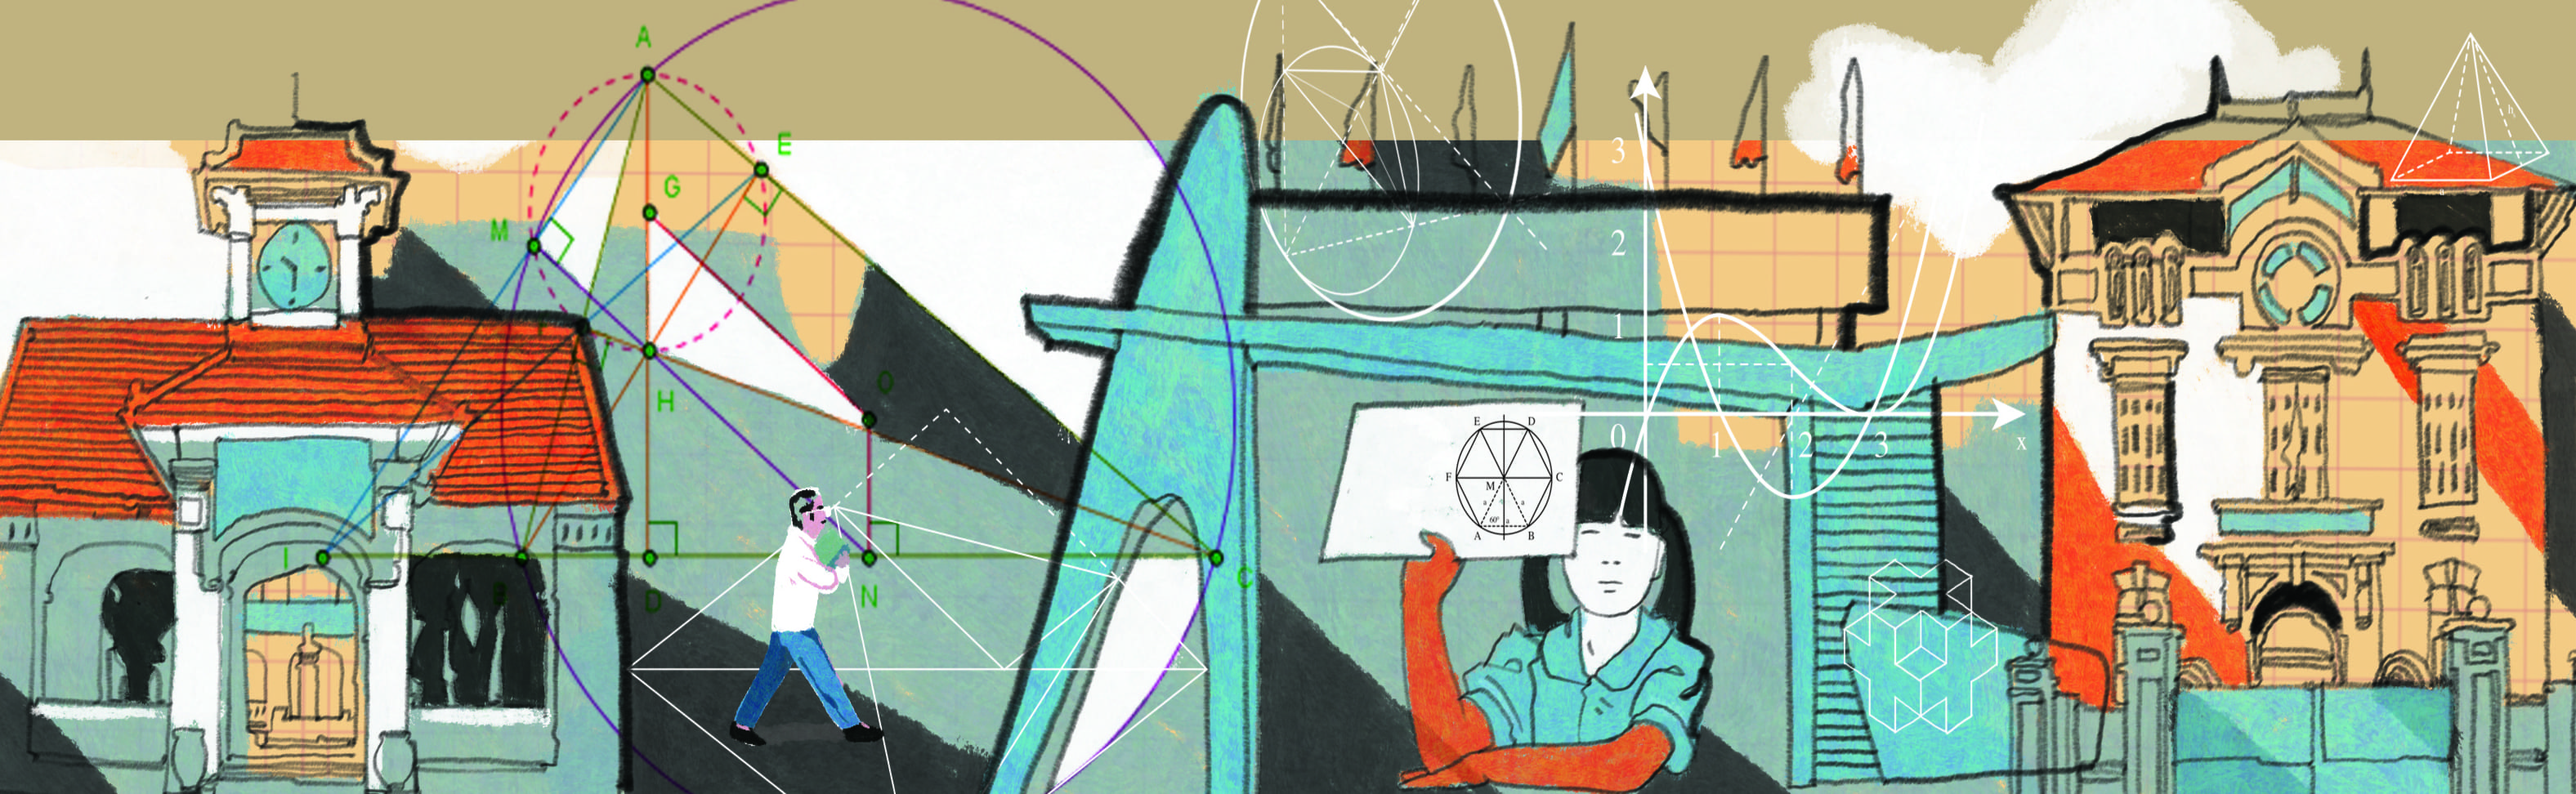
\includegraphics[width=19.3cm]{../bannerdoisong}}}
\AddToShipoutPicture*{\put(86,490){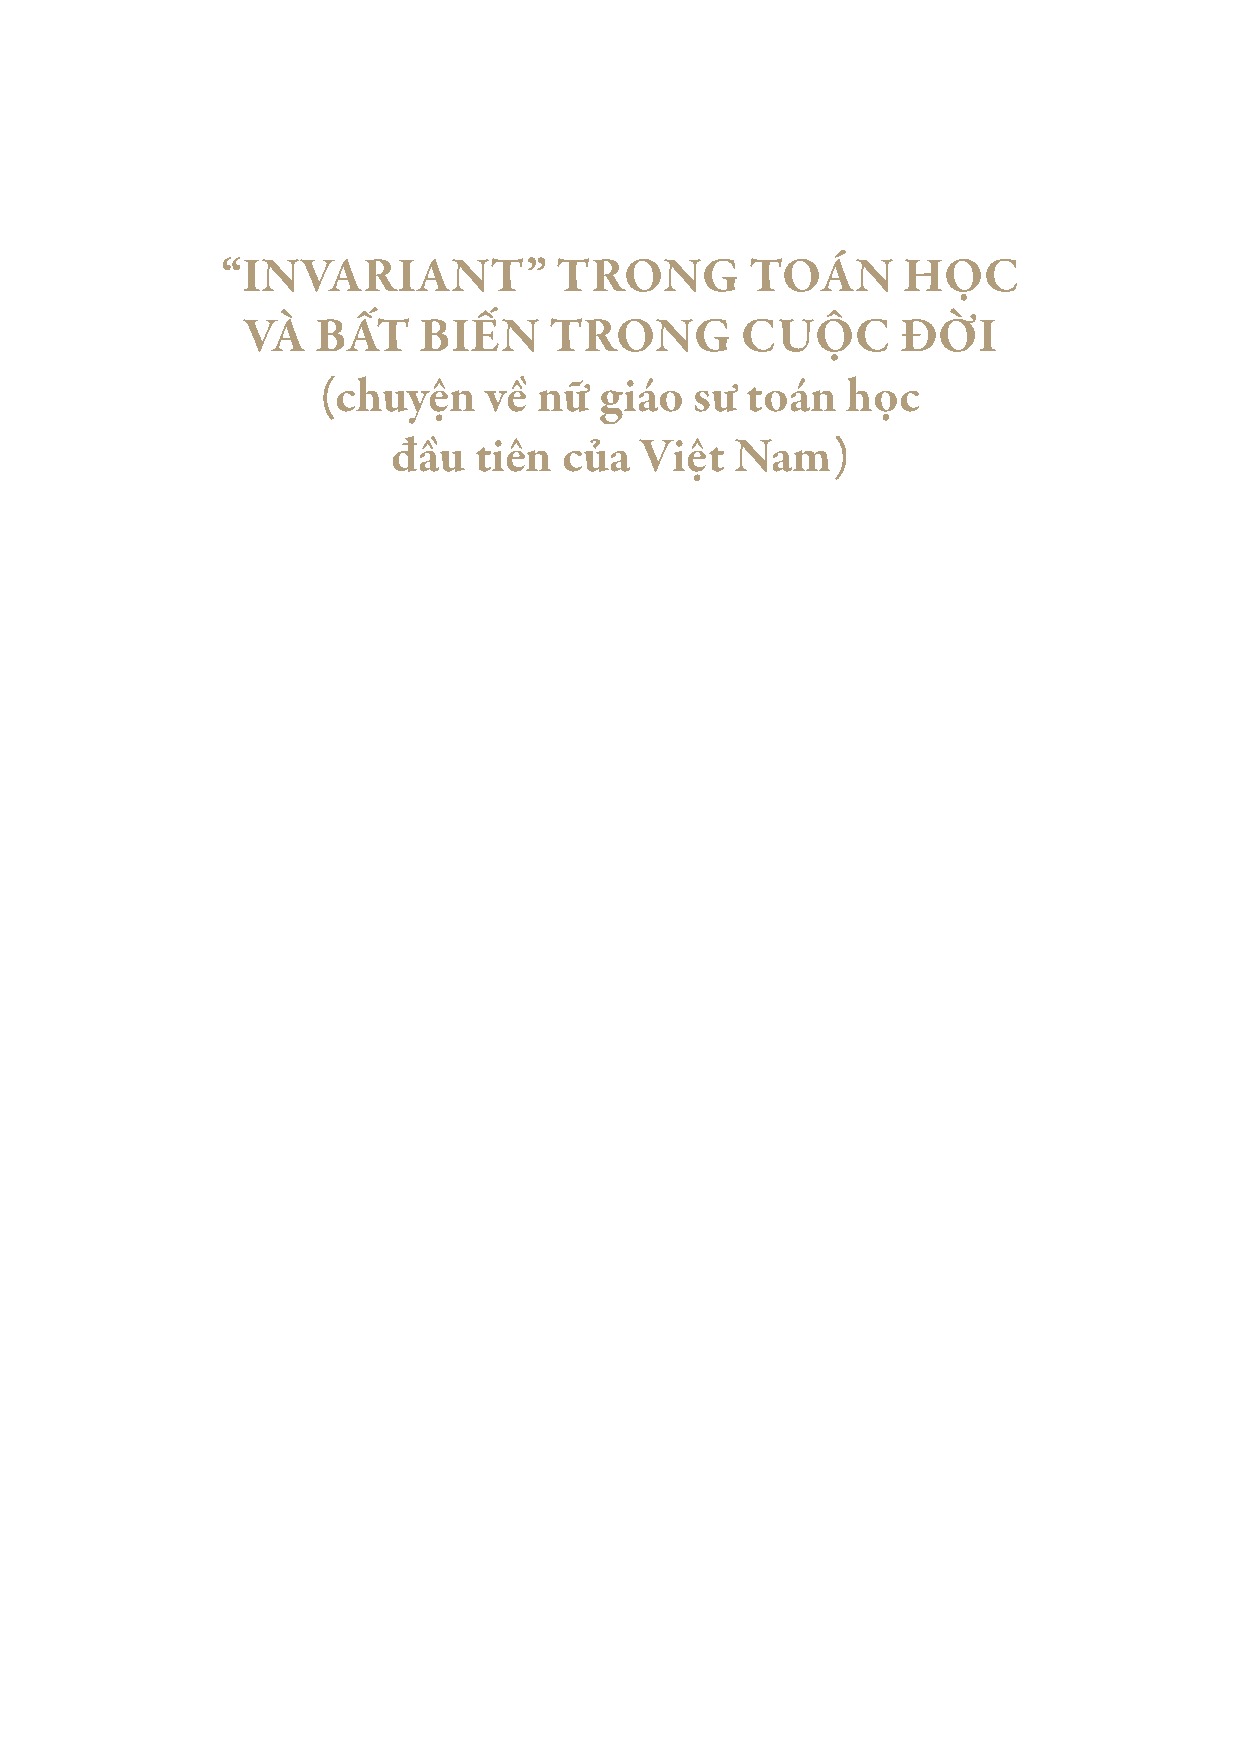
\includegraphics[scale=0.95]{../tieude.pdf}}}\centering
\endgroup

\vspace*{215pt}

\begin{multicols}{2}
	\textbf{\color{doisongtoanhoc}I. Sơ lược tiểu sử}
	\vskip 0.1cm
	Giáo sư Hoàng Xuân Sính sinh ngày $5/9/1933$, là người gốc Làng Cót, Từ Liêm, Hà Nội. Khoảng những năm $40$, gia đình Bà sinh sống tại $102$ Hàng Bông, và ngôi nhà của gia đình Bà cũng chính là cơ sở xuất bản tờ báo Thanh Nghị, tiếng nói của trí thức yêu nước thời bấy giờ.
	\begin{figure}[H]
		\vspace*{-5pt}
		\centering
		\captionsetup{labelformat= empty, justification=centering}
		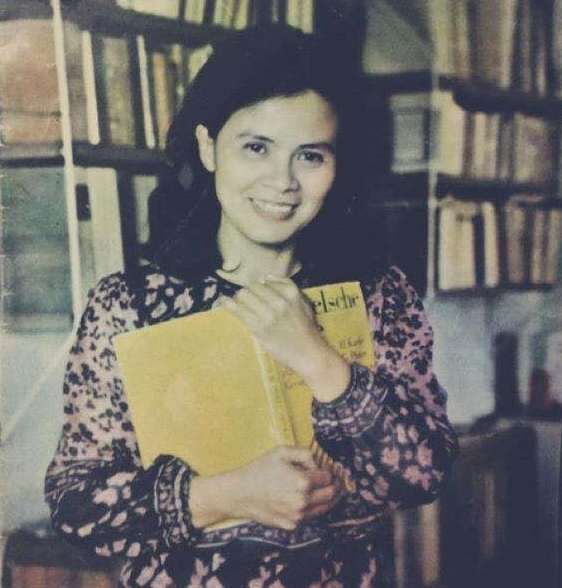
\includegraphics[width= 1\linewidth]{Anh1}
%		\caption{\small\textit{\color{doisongtoanhoc}}}
		\vspace*{-15pt}
	\end{figure}
	Tốt nghiệp trường trung học Chu Văn An năm $1951$, Bà được người cậu ruột đón sang học tiếp ở Pháp. Sau khi nhận bằng Cử nhân Toán học của Đại học Toulouse năm $1957$ và bằng Thạc sĩ Toán học năm $1959$, bà trở về nước đầu năm $1960$.
	\vskip 0.1cm
	``\textit{Tôi đã chọn con đường của nhiều trí thức yêu nước cùng thời, nhớ tới lời dạy của Bác Hồ đối với anh chị em Việt kiều: ``Mỗi người cố học giỏi lấy một nghề, sau này trở về phục vụ Nhân dân". Những lúc Tổ quốc gian khó nhất, là những khi Nhân dân cần chúng ta nhất. Tôi biết, trở về chính là yêu nước}".
	\vskip 0.1cm
	Năm $1975$ Bà bảo vệ Luận án Tiến sĩ quốc gia tại Paris, Pháp. Bản luận án ``Gr--Catégories" của bà là điểm khởi đầu của lý thuyết ``$n$--Catégories", một lý thuyết đang phát triển mạnh trên thế giới, có nhiều ứng dụng trong Vật lý và khoa học tính toán. 
	\vskip 0.1cm
	Năm $1980$, bà được phong học hàm Giáo sư, và là nữ Giáo sư toán học đầu tiên của Việt Nam.
	\vskip 0.1cm
	Năm $1998$, cùng với một số nhà Toán học, bà thành lập Trung tâm đại học Thăng Long, cơ sở giáo dục đại học ngoài công lập đầu tiên của Việt Nam, tiền thân của Trường Đại học Thăng Long. 
	\vskip 0.1cm
	\textbf{\color{doisongtoanhoc}II. Bản luận án ``Gr-Catégories" }
	\vskip 0.1cm
	\textit{$1$. Gr--Categories.}
	\vskip 0.1cm
	Trong Toán học, Hoàng Xuân Sính nổi tiếng với những kết quả trong lý thuyết phạm trù. Và cũng hơi có phần nghịch lý, khi hình như ở nước ngoài người ta biết rõ hơn công đồng toán học trong nước về những đóng góp của Hoàng Xuân Sính! Cũng có thể vì bà hầu như không nhắc đến những kết quả của mình.
	\vskip 0.1cm
	Phần này có mục tiêu giới thiệu sơ lược với những độc giả không là chuyên gia ngành Toán về lý thuyết Gr--Phạm trù và vị trí của nó trong toán học. Đây thực sự là nhiệm vụ rất khó khăn, bởi lẽ Gr--Phạm trù là một lý thuyết rất sâu, không dễ tiếp cận ngay với những nhà toán học không trong chuyên ngành.  
	\vskip 0.1cm
	Trước tiên, xin đưa ra một định nghĩa không hình thức của \textit{phạm trù}.
	Khi mô tả bất kỳ một cấu trúc toán học nào, thậm chí bất kỳ một hiện tượng tự nhiên hay xã hội nào, ta đều cần chỉ ra hai điều mấu chốt: các \textit{đối tượng} được xét trong đó và \textit{quan hệ} giữa chúng.  
	\begin{figure}[H]
		\vspace*{-5pt}
		\centering
		\captionsetup{labelformat= empty, justification=centering}
		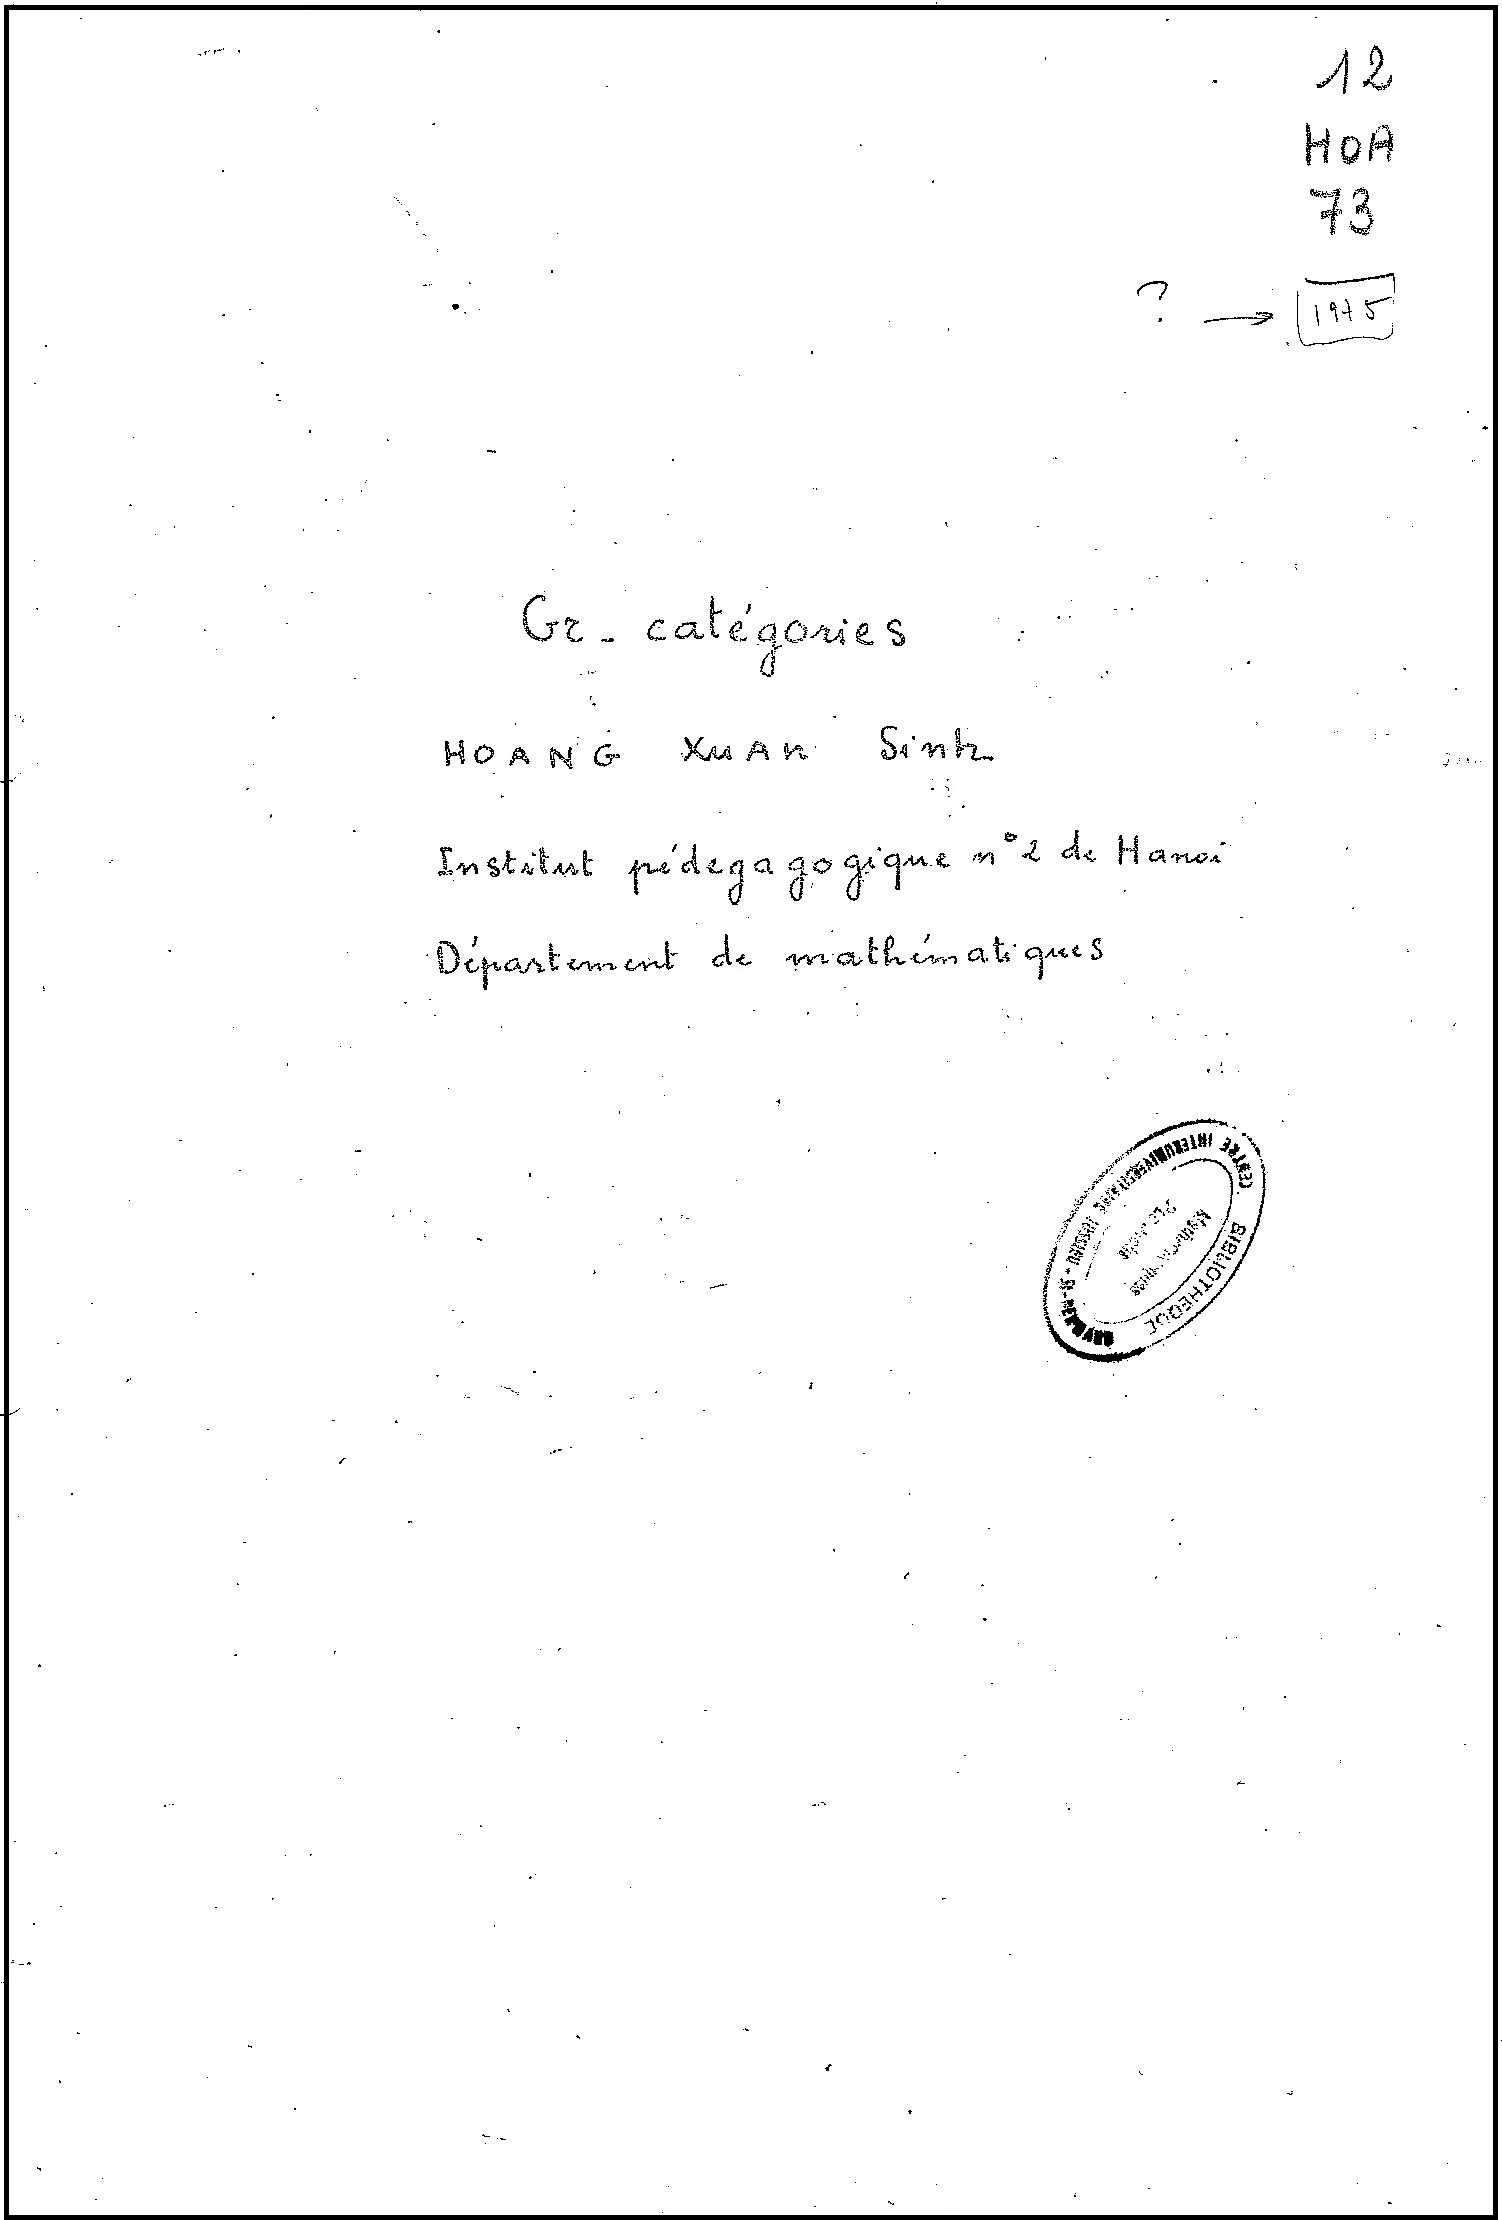
\includegraphics[height= 0.72\linewidth]{Anh21}
		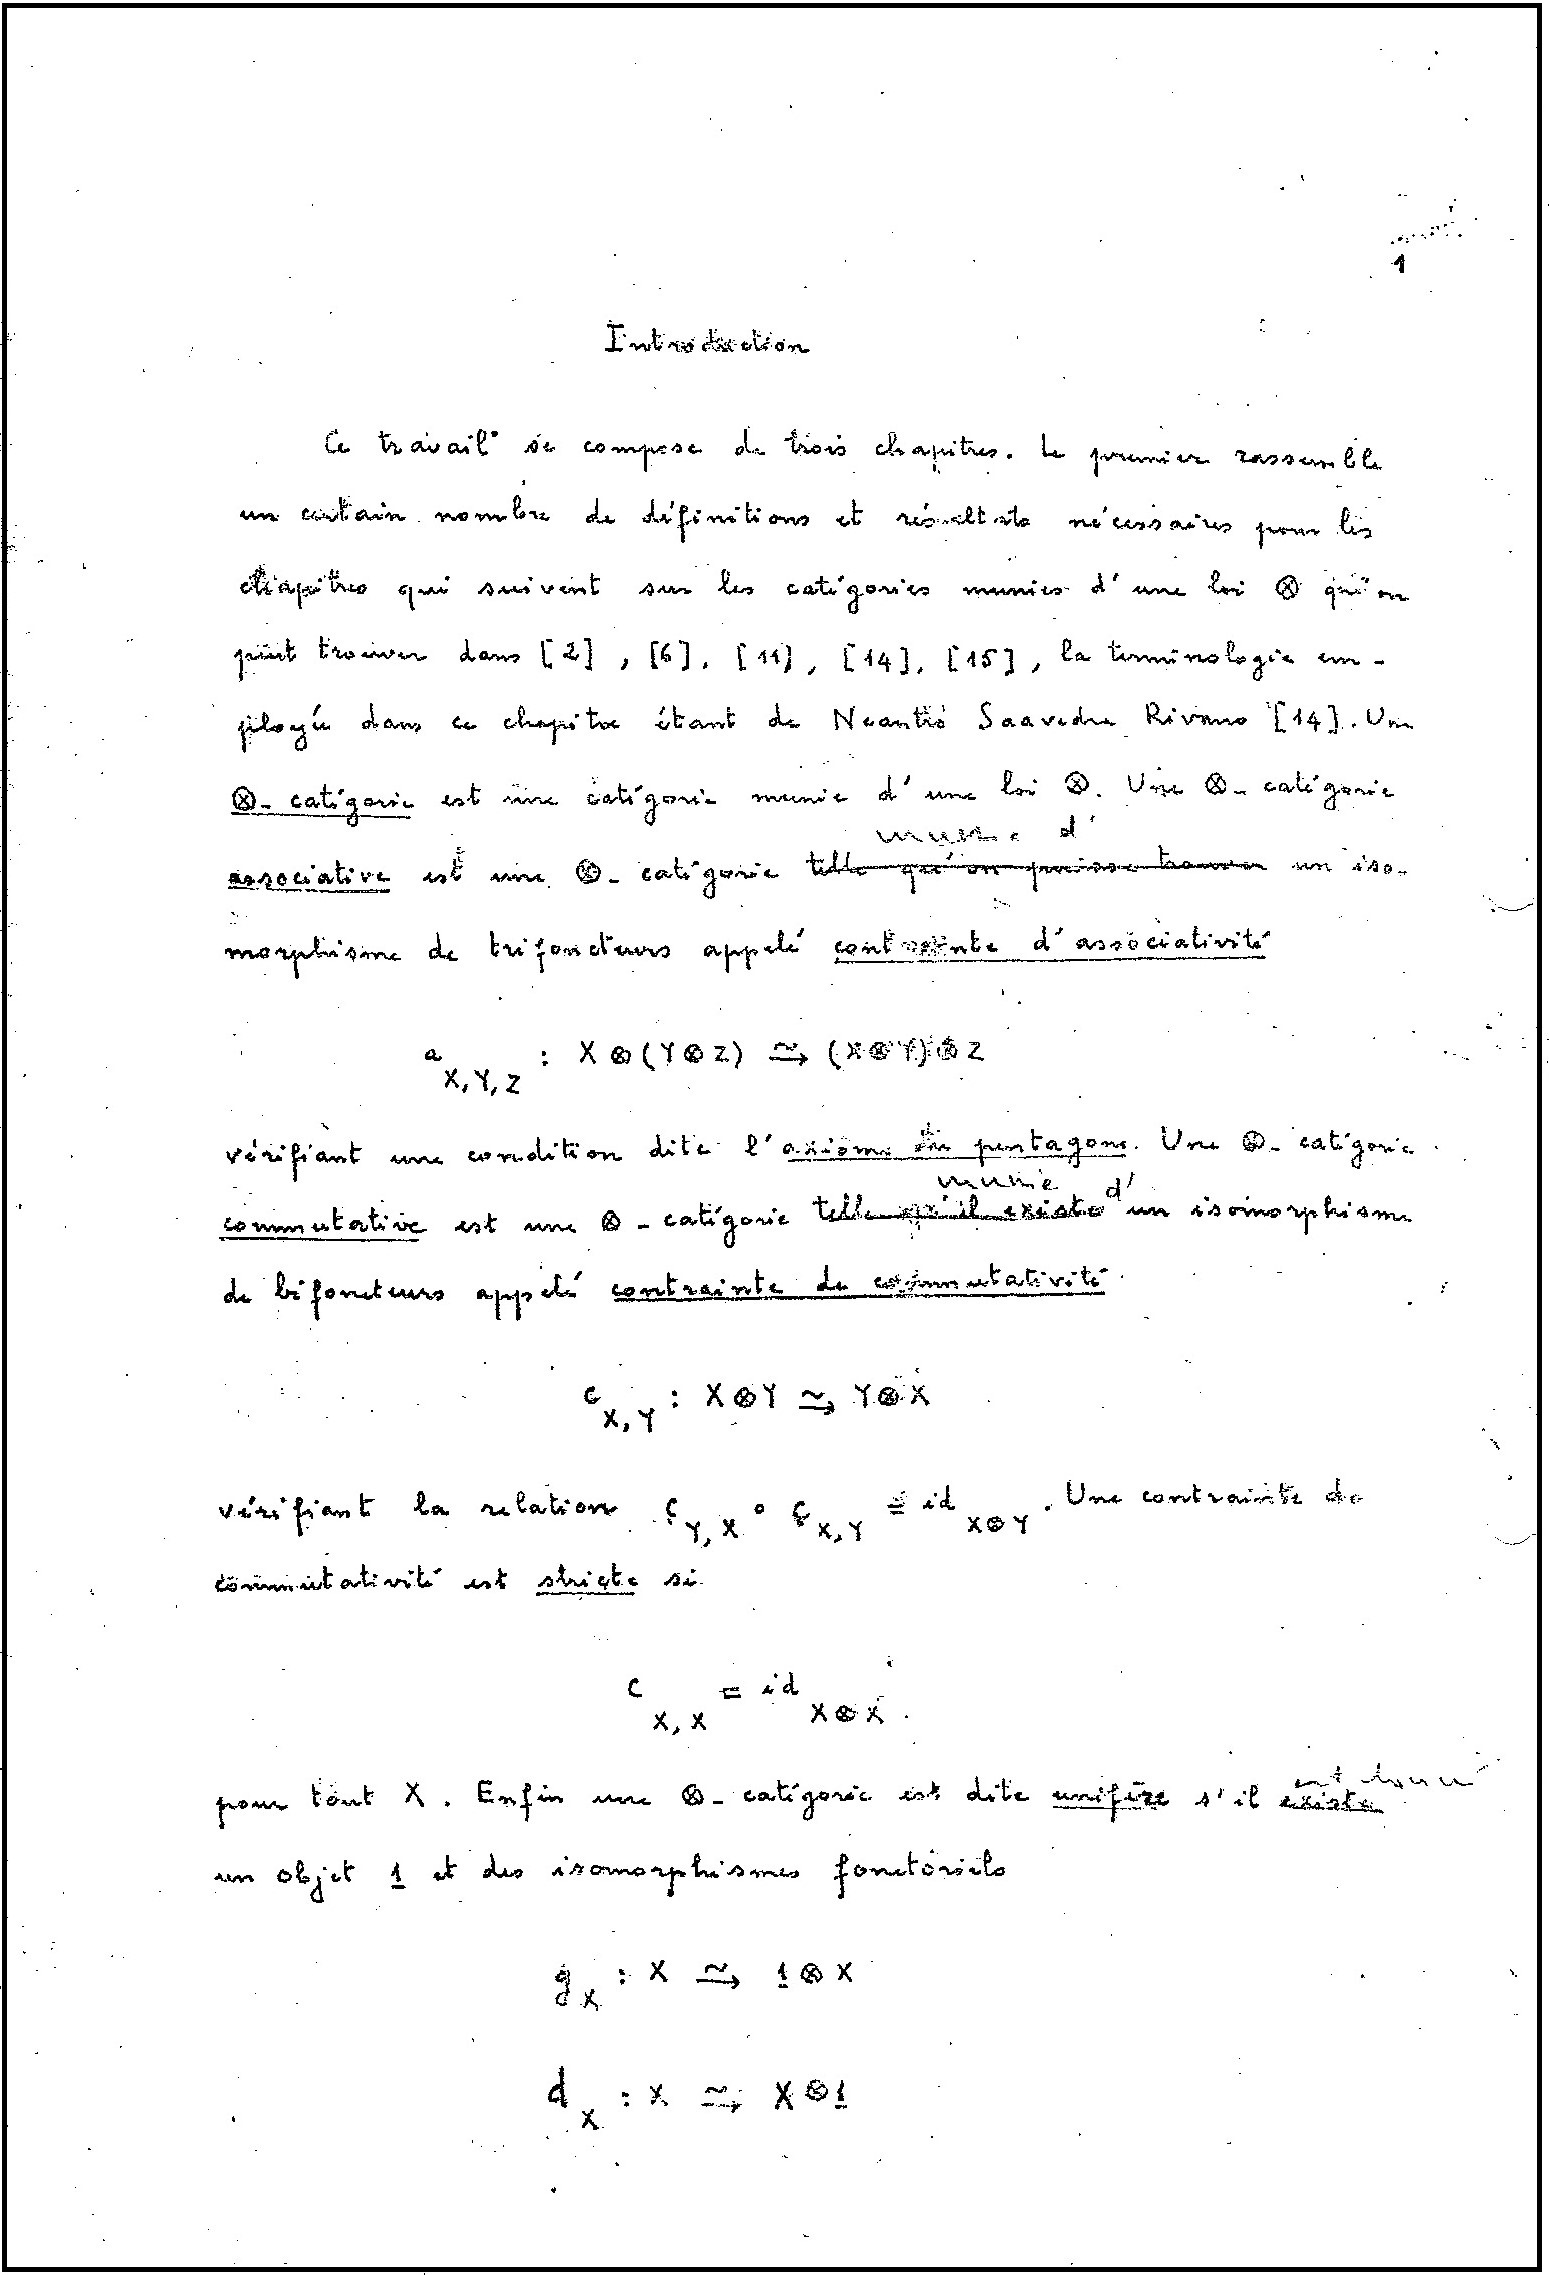
\includegraphics[height= 0.72\linewidth]{Anh22}
		%		\caption{\small\textit{\color{doisongtoanhoc}}}
		\vspace*{-10pt}
	\end{figure}
	Lý thuyết phạm trù ra đời nhằm cung cấp một ngôn ngữ tổng quát để nghiên cứu các cấu trúc toán học. Các đối tượng nghiên cứu ở đây được gọi là các ``vật", quan hệ giữa các vật được cho bởi những ``mũi tên" đi từ vật này đến vật khác. Nói đơn giản, phạm trù là một cặp gồm tập hợp các VẬT (Objects), và tập hợp các MŨI TÊN giữa các  vật, gọi là các ``cấu xạ" (Morphism).
	\vskip 0.1cm
	
	Có thể chỉ ra vài ví dụ:
	\vskip 0.1cm
	$1$/ \textit{Trong Vật lý}. Tập hợp các \textit{trạng thái} của một  hệ vật lý nào đó lập thành tập hợp các ``vật". Quá trình \textit{chuyển trạng thái} cho ta ``cấu xạ" giữa các ``vật".
	\vskip 0.1cm
	$2$/ \textit{Trong Tin học}. Các bộ \textit{dữ liệu} làm thành tập hợp các vật. Chương trình là một cấu xạ chuyển bộ dữ liệu này thành bộ dữ liệu khác.
	\vskip 0.1cm
	$3$/ \textit{Trong Logic}. Các \textit{Mệnh đề} lập thành tập hợp các vật, \textit{chứng minh} là cấu xạ từ mệnh dề này đến mệnh đề khác.
	\vskip 0.1cm
	Như vậy, hầu hết cấu trúc trong toán học, và rộng hơn, trong tự nhiên và xã hội, có thể mô tả bằng ngôn ngữ phạm trù. Tuy nhiên, cũng chính vì phạm trù là cấu trúc quá tổng quát nên từ những kết quả của lý thuyết phạm trù, khó suy ra được những kết quả sâu sắc của các đối tượng thuộc những cấu trúc toán học khác. Vì thế, một yêu cầu tự nhiên là cần đưa vào cấu trúc phạm trù những phép toán nào đó để nó vẫn đủ tổng quát, nhưng có thể chứa đựng, và hơn nữa,  phát hiện những kết quả sâu sắc, chứ không chỉ đóng vai trò như một ngôn ngữ mô tả.
	\vskip 0.1cm
	Một trong những cấu trúc toán học quan trọng nhất là \textit{Nhóm}. Khởi đầu từ công trình của Evariste Galois, lý thuyết nhóm đã trở thành công cụ không thể thiếu trong vật lý. Giáo sư Hoàng Xuân Sính đã đưa ra khái niệm \textit{Gr--phạm trù} và mô tả cấu trúc của chúng. Nói một cách ngắn gọn,  Gr--phạm trù là một phạm trù trong đó trang bị phép tính với ràng buộc kết hợp, đồng thời các vật và các cấu xạ đều có tính chất khả nghịch. Do đó, Gr--phạm trù ``giống như" một nhóm (chữ ``Gr" xuất phát từ ``Group", là \textit{nhóm}). John Baez, nhà toán học và vật lý nổi tiếng viết bài giới thiệu với nhan đề ``\textit{Hoang Xuan Sinh’s thesis: categorifying Group Theory}" (Thang Long Journal of Mathematics and Mathematical Sciences, Vol.$3$, N--$1$, $2023$)
	\vskip 0.1cm
	$2$. \textit{Sính's Invariant.}
	\vskip 0.1cm
	Một bài toán lớn trong Toán học, cũng như trong những ngành khoa học khác, là bài toán phân loại. Để xác định một đối tượng có những tính chất cơ bản gì, chúng ta cần biết chúng thuộc loại nào. Điều này chỉ làm được nếu tìm ra thuộc tính của các đối tượng cùng một  loại, tức là tìm ``bất biến" của lớp đối tượng đó. Nếu một đối tượng mang ``bất biến" của lớp nào, ta biết nó thuộc lớp đó,  tương tự như vân tay là ``bất biến" để nhận biết mỗi người.
	\vskip 0.1cm
	Trong luận án của mình, Giáo sư Hoàng Xuân Sính đã tìm ra một bất biết để nhận biết một lớp các không gian ``đủ tốt", gọi là các \textit{CM--complex}. Cụ thể hơn, khi cho một Gr--phạm trù, ta được hai nhóm: nhóm $G$ các lớp đẳng cấu của các vật, và nhóm $A$ các tự đẳng cấu của vật đơn vị (cũng vì thế, ngày nay người ta gọi Gr--phạm trù là $2$--\textit{nhóm}, và phát triển lý thuyết này thành lý thuyết các \textit{$n$--nhóm}). Một Gr--phạm trù có thể đặc trưng hoàn toàn bởi lớp [$a$] trong nhóm đối đồng điều $H^3(G, A)$. Lớp này ngày nay được mang tên là \textit{Bất biến Sính} (Sính invariant).
	\vskip 0.1cm
	Theo John Baez, một nhà toán học nổi tiếng, ``\textit{kết quả của Hoàng Xuân Sính rọi ánh sáng lên vấn đề nghiên cứu kiểu đồng luân của các không gian tương đối ``đẹp", chẳng hạn các CW--complex}".   
	\vskip 0.1cm
	Hướng nghiên cứu mà giáo sư Hoàng Xuân Sính khởi đầu từ những năm $1967-1975$ ngày nay đang phát triển mạnh, gọi là $n$--phạm trù ($n$--\textit{Category}). Gần đây, những kết quả trong lý thuyết $n$--category được sử dụng trong tính toán lượng tử, cơ sở lý thuyết của các máy tính lượng tử trong tương lai.
	\vskip 0.1cm
	Lý thuyết Gr--Phạm trù được xây dựng trong bản luận án \textit{Gr--Catégories} của Giáo sư Hoàng Xuân Sính, một bản luận án có số phận đặc biệt trong lịch sử toán học. 
	\vskip 0.1cm
	Trong đợt làm việc tại Việt Nam cuối năm $1967$, A. Grothendieck -- một trong những nhà toán học vĩ đại nhất thế kỷ XX -- gợi ý GS Hoàng Xuân Sính nghiên cứu xây dựng một kiểu phạm trù sao cho nó gần như một nhóm. Ý tưởng của Grothendieck được thực hiện thành công, và Gr--Catégories ra đời. Thực ra, ý đồ của Grothendieck xa hơn nhiều: trong tài liệu dày $600$ trang (\textit{Pursuing Stacks}, $1984$. arXiv:$2111.010000$) Grothendieck đưa ra \textit{giả thuyết đồng luân} như sau: ``\textit{Một CW--complex $X$ gọi là kiểu $n$ nếu nhóm $\pi_k(X)$ là tầm thường với $k > n$. Có thể phân lớp sai khác tương đương đồng luân các CW kiểu $n$ bởi các cấu trúc gọi là $n$--nhóm}". Cho đến nay, mới có hai trường hợp được thực hiện hoàn chỉnh là $n =1$ với phạm trù monoidal của Eilenberg-- Mac Lane và  $n = 2$ trong luận án của Giáo sư Hoàng Xuân Sính. Trường hợp $n > 2$ vẫn đang được quan tâm nghiên cứu và mới có những kết quả riêng rẽ.
	\begin{figure}[H]
		\vspace*{-5pt}
		\centering
		\captionsetup{labelformat= empty, justification=centering}
		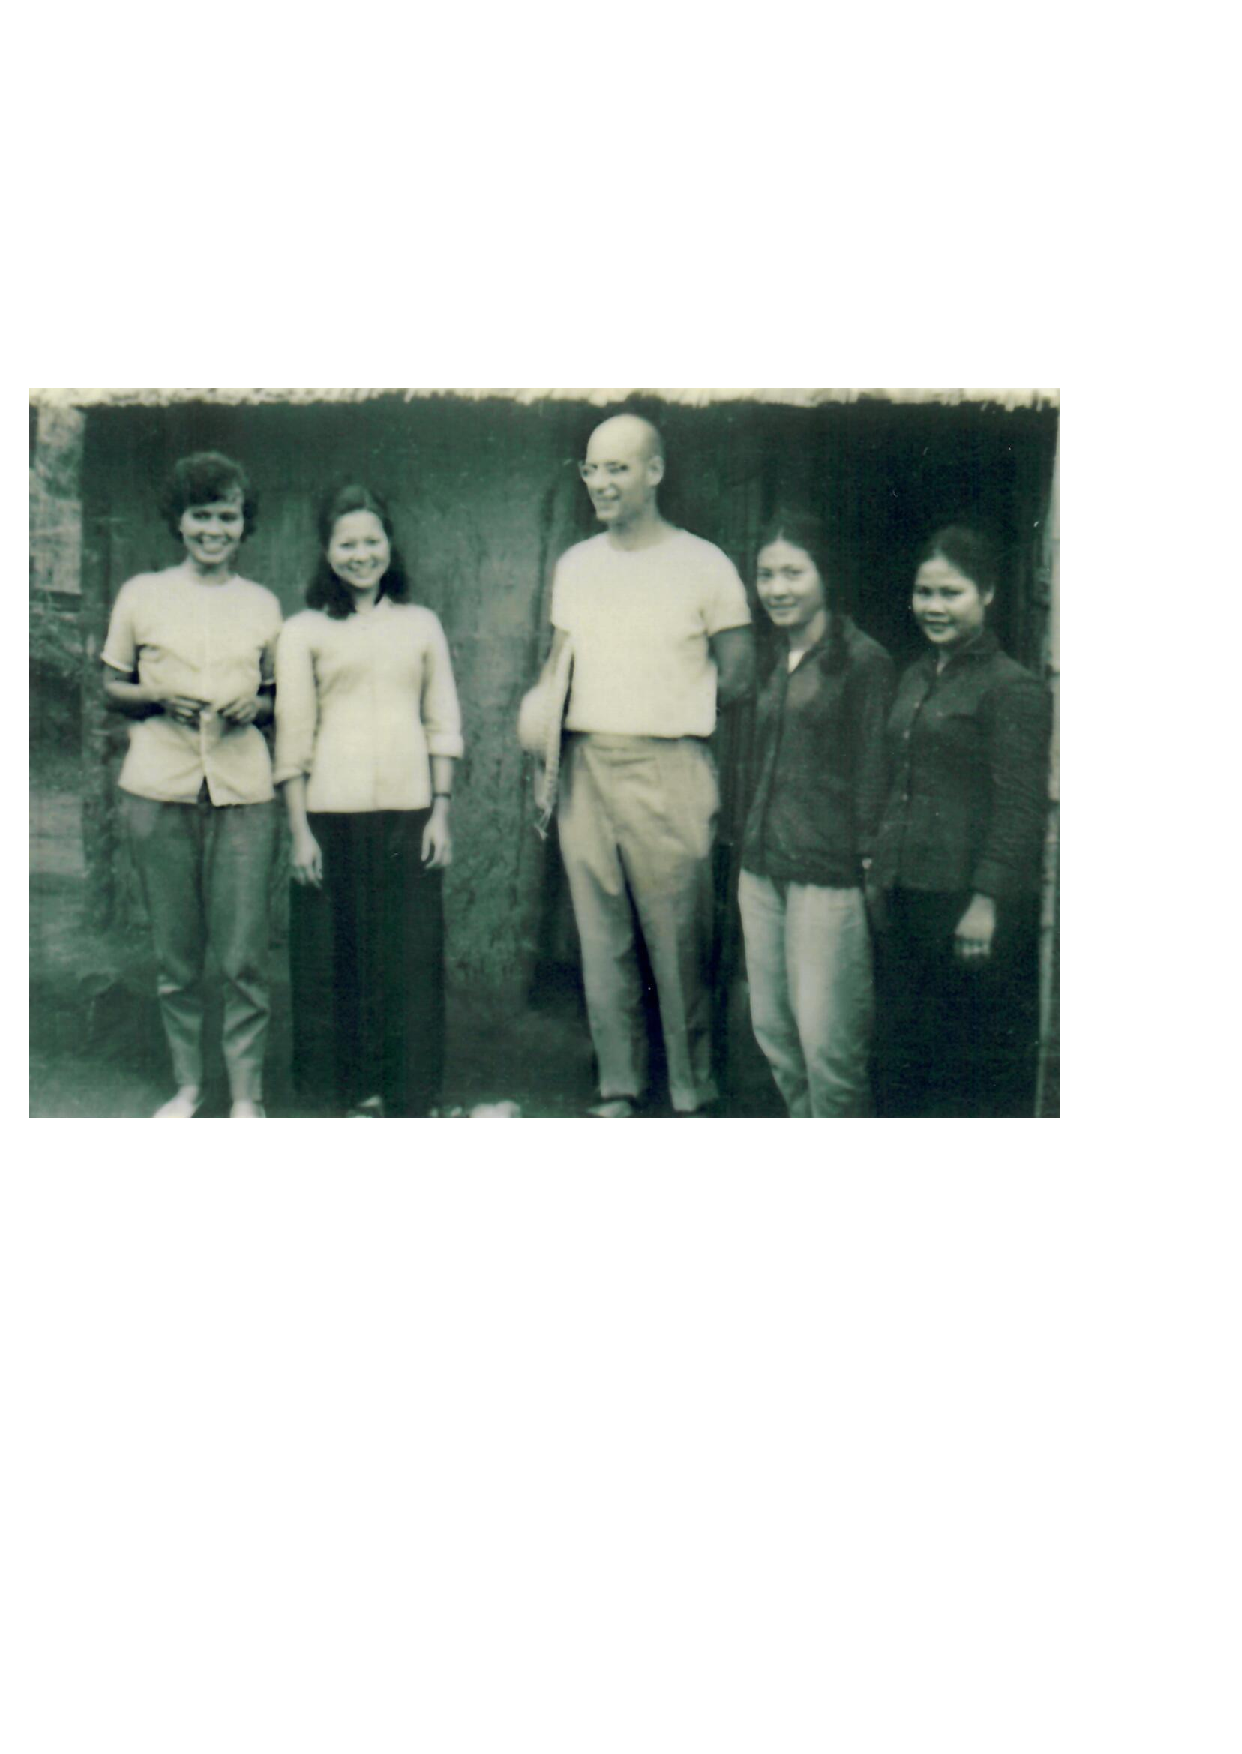
\includegraphics[width= 1\linewidth]{Anh3}
%		\caption{\small\textit{\color{doisongtoanhoc}}}
		\vspace*{-10pt}
	\end{figure}
	Trong suốt thời gian làm luận án, GS Hoàng Xuân Sính chỉ liên hệ với Grothendieck $3$ lần, qua những bức thư ngắn chỉ đến được với người nhận sau hơn nửa năm! Thật khó tìm được luận án tiến sĩ nào khác trên thế giới được viết trong chiến tranh, trong điều kiện hoàn toàn cô lập với thế giới toán học, không có nhóm nghiên cứu, thiếu tài liệu, và thậm chí thiếu cả những điều kiện tối thiểu như giấy bút, ánh sáng và những bữa ăn no! Giáo sư Hàng Xuân Sính kể rằng, khi ở khu sơ tán, ước mơ của bà nhiều khi chỉ là làm sao có đủ pin để ngồi làm việc trong màn, tránh được đàn mỗi dày đặc quanh chiếc đèn dầu!
	\vskip 0.1cm
	Bản luận án ``Gr--Catégories" làm thế giới toán học quan tâm và ngạc nhiên, không chỉ vì nội dung, mà còn ở sự ra đời đặc biệt của nó. 
	\vskip 0.1cm
	Luận án được hoàn thành năm $1973$, và bản \textit{viết tay} của nó được gửi cho Grothendieck. Sau nhiều trắc trở, năm $1975$ Hoàng Xuân Sính được phép ghé Paris trên đường trở về từ Đại hội toán học thế giới ở Vancouver để bảo vệ luận án Tiến sĩ quốc gia. Hội đồng chấm luận án của Bà cũng thật hiếm thấy, khi gồm những nhà toán học nổi tiếng nhất: H. Cartan, A. Grothendieck,  J. L. Verdier, L. Schwartz, M. Zisman.
	\vskip 0.1cm
	Những tháng gần đây, nhân sinh nhật lần thứ $90$ của Giáo sư Hoàng Xuân Sính,   trên báo chí có nhiều có nhiều bài viết về ``sự trở về kỳ diệu" của bản luận án viết tay \textit{Gr--Catégories}. Tuy nhiên, với những nhà toán học thì sự trở về kỳ diệu chỉ thực sự xẩy ra khi những kết quả của họ được nhắc đến, được tiếp tục phát triển sau hơn nửa thế kỷ! Bản luận án của Giáo sư Hoàng Xuân Sính đã trở về, và ở lại mãi mãi với toán học, trong những nghiên cứu về \textit{Sính invariant và $n$--Categories.}
	\vskip 0.1cm
	Xin dẫn vài lời đánh giá của  J. Baez:
	\vskip 0.1cm
	``\textit{Sẽ là thiếu sót nếu không đề cập đến việc các Gr--Phạm trù,  ngày nay thường được gọi là $2$--nhóm,  đã có một sức sống mới trong vật lý lý thuyết và toán học.
	\vskip 0.1cm
	Lý do là vì Lý thuyết trường chuẩn (Gauge Theory), cách tiếp cận thành công ngoạn mục của vật lý dựa trên các nhóm, có thể được khái quát hóa thành lý thuyết trường chuẩn bậc cao bằng cách sử dụng $2$--nhóm.
	\vskip 0.1cm
	Hơn nữa, không có lý do gì để dừng lại ở $2$ nhóm ... Có những hy vọng rằng một ngày nào đó các nhà vật lý sẽ tổng hợp các pha của vật chất được mô tả bởi lý thuyết trường chuẩn bậc cao. Đó sẽ là sự hiện thực hóa tuyệt vời tầm nhìn của Hoàng Xuân Sinh.}"
	\vskip 0.1cm
	\columnbreak
	Những năm sau này, GS Hoàng Xuân Sính không còn thời gian dành cho nghiên cứu toán học, khi dồn hết sức lực và tâm huyết để xây dựng Trường Đại học Thăng Long. 
	\begin{figure}[H]
		\vspace*{-5pt}
		\centering
		\captionsetup{labelformat= empty, justification=centering}
		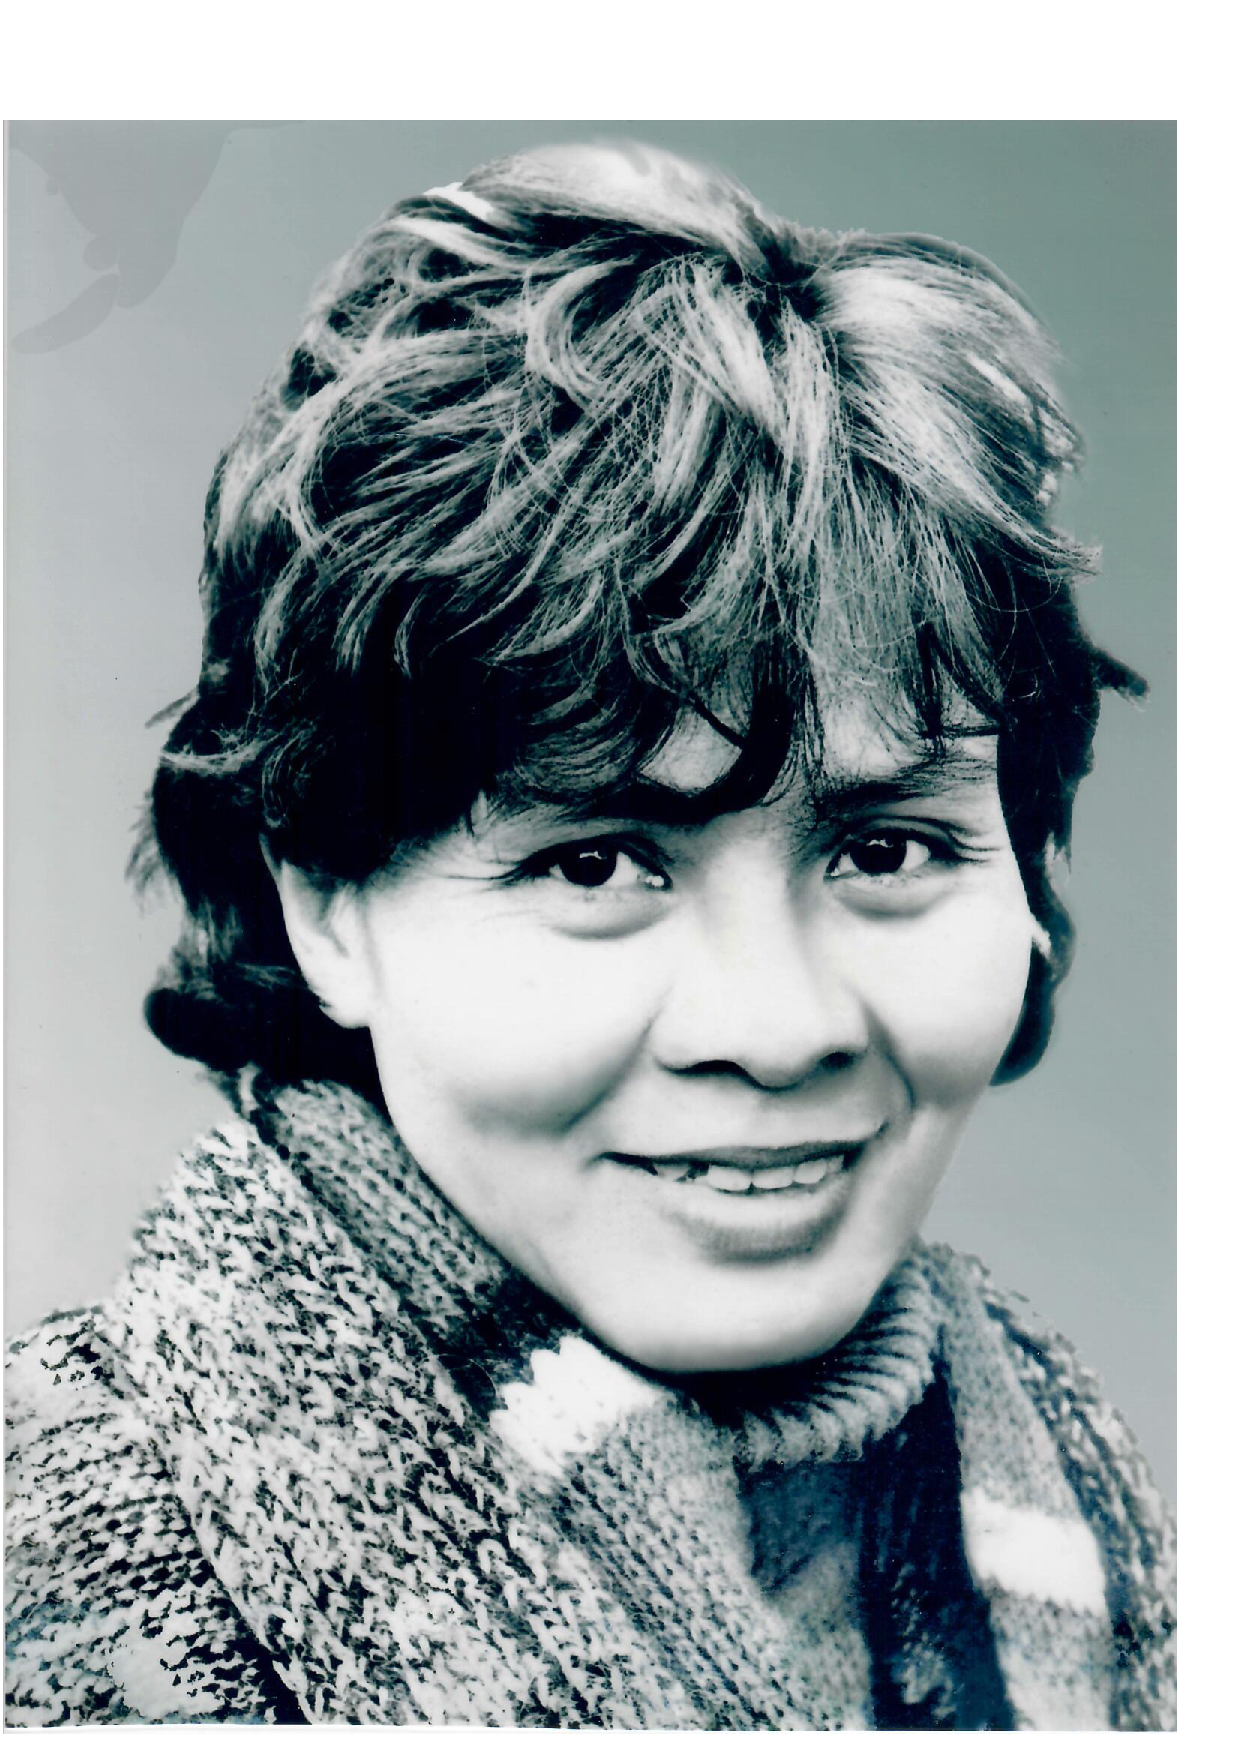
\includegraphics[width= 1\linewidth]{Anh12}
		\caption{\small\textit{\color{doisongtoanhoc}}}
		\vspace*{-20pt}
	\end{figure} 
	Cuộc đời Bà là hành trình nhất quán của một trí thức yêu nước và nhà khoa học đầy tài năng: từ quyết định rời bỏ cuộc sống tiện nghi ở nước Pháp để trở về đóng góp cho nền giáo dục Việt Nam trong những năm chiến tranh ác liệt, quyết tâm vươn lên đỉnh cao khoa học trong những điều kiện đặc biệt khó khăn, cho đến những cố gắng và nghị lực phi thường để vượt qua biết bao thử thách, xây dựng trường đại học ngoài công lập đầu tiên trong hệ thống giáo dục của Việt Nam.
	\vskip 0.1cm
	Nếu như trong toán học, ``bất biến Sính" (\textit{Sính' Invariant}) là một lớp đối đồng điều, thì ``bất biến Sính" trong cuộc đời chính là tình yêu của Bà với Tổ Quốc và Khoa Học. 
\end{multicols}